\documentclass[11pt,a4paper]{article}
\usepackage[utf8]{inputenc}
\usepackage[T1]{fontenc}
\usepackage[margin=2.5cm]{geometry}
\usepackage{amsmath,amssymb}
\usepackage{graphicx}
\usepackage{booktabs}
\usepackage{siunitx}
\usepackage{microtype}
\usepackage{float}
\usepackage{xcolor}
\usepackage[font=small,labelfont=bf]{caption}
\usepackage[authoryear,round]{natbib}
\usepackage[colorlinks=true,linkcolor=blue!50!black,citecolor=blue!50!black,urlcolor=blue!50!black]{hyperref}
\usepackage[capitalise,noabbrev]{cleveref}

\graphicspath{{../figures/}}

\title{Did a Teacher Platform Raise Grades?\\ A Re-analysis of the ClassRoomMate Pilot}
\author{Juan Carlos Chavarr\'ia Morales\\[2pt]
  \small M.Sc.\ Optimization, Hochschule Bielefeld (HSBI)}
\date{October 2026}

\begin{document}
\maketitle

\begin{abstract}
In the second semester of 2018, the learning-management platform ClassRoomMate was piloted in a public school in
Santiago, Chile: 51 teachers, 27 classes from 4th grade to the last year of secondary school. Each teacher, together
with the students of each class, chose how intensively to use it. The original evaluation compared the change of the
class mean between the two semesters across usage levels and reported that intensive use raised performance by
\SI{3.5}{\percent} to \SI{6.1}{\percent} and the probability of improvement to \SI{75}{\percent}. We rebuilt the
analysis from the school's grade books. The original numbers replicate exactly, but three of them overstate the
evidence: the \SI{6.1}{\percent} is an average over the improving classes only, the \SI{75}{\percent} counts
unchanged classes as improved, and the classes that chose intensive use started from a lower mean, so part of their
gain is regression to the mean. Adjusted for the starting level and for the clustering of classes within teachers,
intensive use is associated with a change of $+1.2\%$ (95\% CI $-1.3\%$ to $+3.6\%$), which is compatible with
no effect as well as with a small positive one. With 13 to 15 intensive-use teachers, the pilot could only have
detected differences of about \SI{4}{\percent}. Because usage was self-selected and the outcome is the grades given
by the same teachers, the data support an association at most, not an impact.
\end{abstract}

% =====================================================================================================================
\section{Context and question}

ClassRoomMate is a platform for teachers: it records assessments, follows the progress of each class and gives
feedback to students. In the second semester of 2018 it was piloted in a municipal (public) school in Santiago, Chile,
in all classes from 4th grade of primary school (\emph{básica}) to the 4th year of secondary school (\emph{media}).
The pilot covered 27 classes and 329 class--subject combinations (152 in primary, 177 in secondary school), taught by
51 teachers; religion, orientation and remedial lessons were excluded.

A first evaluation (2019, revised in 2025) compared the change of the class mean between the first and the second
semester across three usage levels (\emph{intensive}, \emph{medium}, \emph{low or none}) and concluded that
intensive use had a positive and significant effect on performance. This report asks whether that conclusion holds:
\begin{enumerate}
  \item Do the original numbers replicate from the original work sheet, and do they mean what the report says?
  \item What remains of the association once the starting level of each class and the dependence between classes of
        the same teacher are taken into account?
  \item What can such a pilot show at all, and how should the next one be designed?
\end{enumerate}

\paragraph{Disclosure.} The author collaborated with ClassRoomMate during the pilot. The data are the school's
grade records; the school is not named, and no personal data are published (\cref{sec:data}).

% =====================================================================================================================
\section{Materials}\label{sec:data}

\paragraph{Outcome.} For every class--subject $i$ (a class taught by one teacher), the ratio of the class means of the
two semesters,
\[
  r_i = \bar x_{2,i} / \bar x_{1,i},
\]
on the Chilean grade scale from 1 to 7. We analyse $\log r_i$, approximately the relative change; $r_i > 1$ means that
the class mean rose.

\paragraph{Usage.} The usage level was decided per teacher and class, by the teacher together with the students of
that class. It is therefore self-selected at the level of the class.

\paragraph{Sources.} The original evaluation worked from a work sheet holding one $r_i$ per class--subject, grouped
in six blocks (primary / secondary $\times$ three usage levels), but without the class each row belongs to. We
recomputed the class means from the school's grade books (one export per class with every student's semester
averages), linked each class--subject to its teacher through the staff list, and replaced the teachers' names by
anonymous identifiers. Each work-sheet row was then located in its class: first by matching its ratio to a
recomputed one (same level and subject; 116 rows), keeping only matches consistent with the class order of the
work sheet, then by filling gaps between two matches of the same class (62 rows). The analysis uses the 142 located
rows with known teacher and baseline: 47 teachers, 24 classes. Low-use classes are somewhat over-represented among
them (\SI{56}{\percent} against \SI{47}{\percent}), but the mean ratio of each usage level is the same as in the full
work sheet (\cref{tab:describe,tab:replication}).

\paragraph{Privacy.} The grade books contain the names and grades of students, most of them minors, and the staff
list contains the teachers' names. Neither is published. The code runs on the school's files and writes only class
means with anonymous teacher identifiers, which stay private as well; the tests use synthetic grade books.

% =====================================================================================================================
\section{Replication of the original analysis}\label{sec:replication}

The original code reproduces the published numbers exactly (\cref{tab:replication}; logistic coefficient for
intensive use 1.040, mixed-model coefficient 0.035, as in the original report). Four points change their reading.

\begin{table}[t]
  \centering\small
  \caption{Original summary by usage level, replicated from the work sheet. The original code kept the summary rows
    of the work sheet (block mean, maximum, minimum) as if they were classes; removing them changes little.
    $P(r \ge 1)$ is the original definition of improvement, $P(r > 1)$ excludes unchanged classes.}
  \label{tab:replication}
  \begin{tabular}{lrrrcr}
\toprule
usage & classes & mean $r$ & $P(r \ge 1)$ [\%] & 95\% CI & $P(r > 1)$ [\%] \\
\midrule
\multicolumn{6}{l}{\emph{original code (summary rows kept)}} \\
\quad intensive & 116 & 1.022 & 74.1 & [66.2, 82.1] & 62.1 \\
\quad medium & 70 & 1.001 & 62.9 & [51.5, 74.2] & 50.0 \\
\quad low / none & 159 & 0.993 & 49.1 & [41.3, 56.8] & 39.6 \\
\multicolumn{6}{l}{\emph{summary rows removed}} \\
\quad intensive & 110 & 1.023 & 74.6 & [66.4, 82.7] & 61.8 \\
\quad medium & 64 & 1.003 & 64.1 & [52.3, 75.8] & 50.0 \\
\quad low / none & 155 & 0.993 & 49.0 & [41.2, 56.9] & 39.4 \\
\bottomrule
\end{tabular}

\end{table}

\begin{enumerate}
  \item \textbf{Summary rows counted as classes.} 16 summary rows of the work sheet (mean, maximum and minimum of each
    block) entered the analysis as classes (345 instead of 329 rows). The effect on the results is small.
  \item \textbf{No change counted as improvement.} Improvement was defined as $r \ge 1$. Because the class means were
    rounded to one decimal, \SI{12}{\percent} of the classes have exactly $r = 1$. Counting only real improvements,
    the share is \SI{62}{\percent} for intensive and \SI{39}{\percent} for low use, instead of 75 and
    \SI{49}{\percent} (\cref{fig:ties}).
  \item \textbf{The \SI{6.1}{\percent} is conditional on improvement.} It is the mean increase over the intensive-use
    classes that improved. The same number for the low-use classes that improved is \SI{4.3}{\percent}; over all
    intensive-use classes, the mean ratio is 1.023, against 0.993 for low use.
  \item \textbf{Inconsistent tables.} The original tables report 110 intensive-use classes in one place and 116 in
    another, and the table of the medium usage level repeats the totals of the intensive one (110 classes, 41
    improving, \SI{37}{\percent}), whereas the work sheet has 64 classes with 41 improving (\SI{64}{\percent}).
\end{enumerate}
Finally, both original models treat the classes as independent observations, or group them by subject. The decision
on usage, however, was taken per teacher and class, so classes of the same teacher are not independent; and neither
model accounts for the level at which a class started.

\begin{figure}[t]
  \centering
  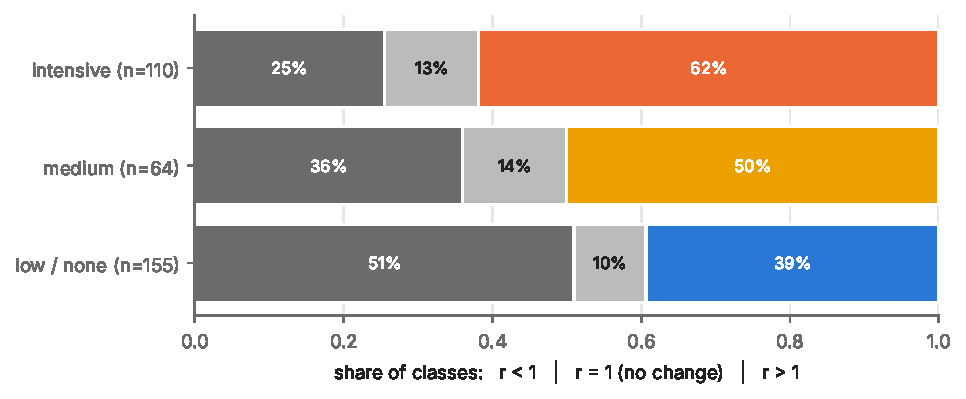
\includegraphics[width=0.8\linewidth]{ties.pdf}
  \caption{Share of classes whose mean fell, stayed the same (rounded to one decimal) or rose, by usage level (all
    329 work-sheet rows).}
  \label{fig:ties}
\end{figure}

% =====================================================================================================================
\section{Re-analysis}\label{sec:reanalysis}

\paragraph{Regression to the mean.} Classes that start with a low mean tend to rise, and classes that start high
tend to fall: one grade point more in the first semester goes with a change of $-4.1\%$ (95\% CI $-6.0\%$ to
$-2.1\%$) in the second. The classes that chose intensive or medium use started 0.35 grade points lower than those
with low use (\cref{tab:describe,fig:baseline}), so part of their gain would have occurred without the platform.

\begin{table}[t]
  \centering\small
  \caption{Located work-sheet rows used in the re-analysis, by usage level.}
  \label{tab:describe}
  \begin{tabular}{lrrrrr}
\toprule
usage & classes & teachers & baseline (sem.\,1) & mean $r$ & $P(r>1)$ [\%] \\
\midrule
intensive & 42 & 15 & 5.63 & 1.022 & 69.0 \\
medium & 21 & 6 & 5.65 & 1.004 & 57.1 \\
low / none & 79 & 29 & 5.98 & 0.993 & 36.7 \\
\bottomrule
\end{tabular}

\end{table}

\begin{figure}[t]
  \centering
  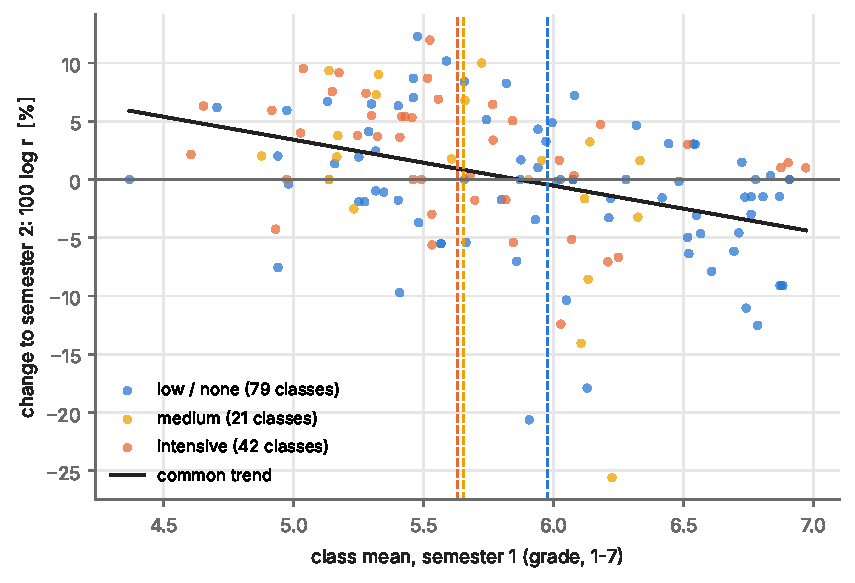
\includegraphics[width=0.8\linewidth]{baseline.pdf}
  \caption{Change of the class mean against its level in the first semester (one point per class--subject). Dashed:
    mean starting level of each usage group. Intensive-use classes started lower and lie on the common trend.}
  \label{fig:baseline}
\end{figure}

\paragraph{Models.} \Cref{tab:models,fig:effects} estimate the same contrast under increasingly careful
specifications. Without adjustment, intensive use goes with $+2.7\%$ ($p = 0.02$), close to the original estimate of
the work sheet. Clustering the standard errors by teacher changes little here; adjusting for the starting level
halves the estimate to $+1.2\%$ and its confidence interval includes zero, whether the classes are clustered by
teacher, by class, or modelled with random effects for both. Medium use shows no association in any specification.

\begin{table}[t]
  \centering\small
  \caption{Difference in the semester change ($100 \log r$) with respect to low use. Baseline: class mean of the
    first semester. All specifications include primary/secondary level.}
  \label{tab:models}
  \resizebox{\linewidth}{!}{\begin{tabular}{lrrrr}
\toprule
specification & \multicolumn{2}{c}{intensive vs low} & \multicolumn{2}{c}{medium vs low} \\ \cmidrule(lr){2-3}\cmidrule(lr){4-5}
& difference [\%] (95\% CI) & $p$ & difference [\%] (95\% CI) & $p$ \\
\midrule
OLS, classes independent & +2.7 [+0.4, +5.1] & 0.023 & +0.7 [$-$2.4, +3.7] & 0.656 \\
OLS, SE clustered by teacher & +2.7 [+0.4, +5.1] & 0.023 & +0.7 [$-$3.0, +4.4] & 0.714 \\
+ baseline, SE clustered by teacher & +1.2 [$-$1.3, +3.6] & 0.363 & $-$0.9 [$-$4.9, +3.2] & 0.674 \\
+ baseline, SE clustered by class & +1.2 [$-$0.9, +3.3] & 0.280 & $-$0.9 [$-$4.9, +3.2] & 0.673 \\
mixed model: teacher + class, + baseline & +1.2 [$-$1.1, +3.4] & 0.316 & $-$0.9 [$-$3.7, +2.0] & 0.551 \\
\bottomrule
\end{tabular}
}
\end{table}

\begin{figure}[t]
  \centering
  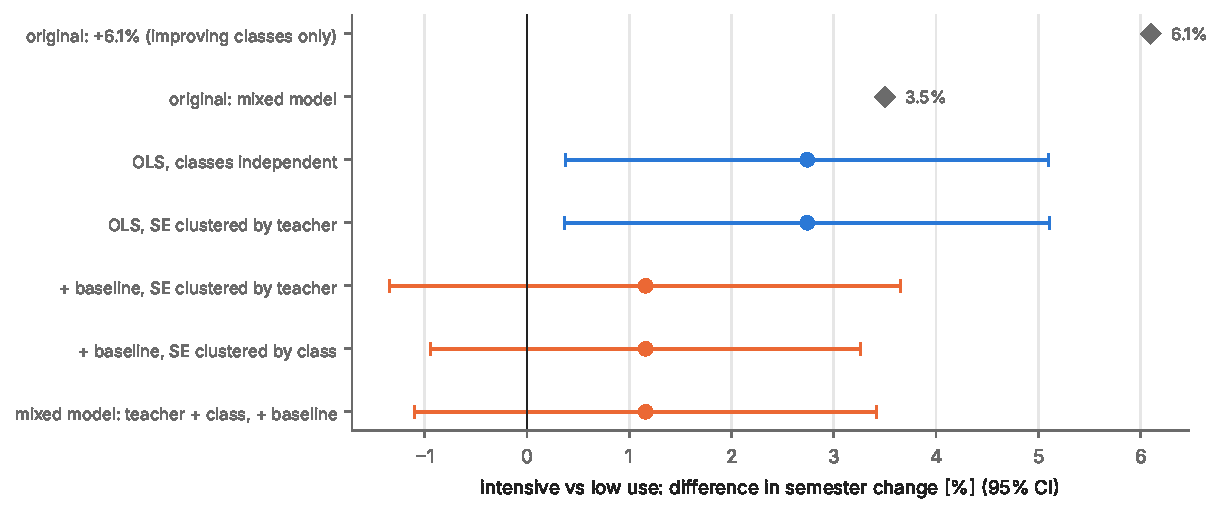
\includegraphics[width=0.9\linewidth]{effects.pdf}
  \caption{Intensive vs low use: the original figures (diamonds) and the estimates of \cref{tab:models} with 95\%
    confidence intervals.}
  \label{fig:effects}
\end{figure}

\paragraph{Teachers as the unit.} Usage was nearly constant per teacher (only 3 of 47 teachers have classes with
different levels). Averaging the baseline-adjusted change per teacher and comparing the 13 intensive-use with the 28
low-use teachers gives a difference of $+1.7\%$; a permutation test of the teachers' labels gives $p = 0.29$.

\paragraph{Power.} With these teachers and the observed spread of their adjusted changes, the smallest difference
that a two-sided test at the 5\,\% level would detect with \SI{80}{\percent} power is about \SI{4.2}{\percent}. The
pilot was too small to detect effects much smaller than those it claimed.

% =====================================================================================================================
\section{What the pilot can and cannot show}\label{sec:limits}

Three features of the design limit any conclusion, independently of the statistics:
\begin{itemize}
  \item \textbf{Self-selection.} Teachers and classes chose their usage level. Motivated teachers or classes may
    adopt the platform and improve for the same reason; the comparison of usage levels mixes the effect of the
    platform with the reasons for choosing it.
  \item \textbf{The outcome is set by the participants.} The grades are given by the same teachers whose usage is
    compared. A platform that structures assessment can change how grades are given, not only how much students learn.
  \item \textbf{No comparison over time or with another school.} Only one semester change is observed; there is no
    record of how the same classes changed in previous years.
\end{itemize}
A pilot that could show an effect would assign the platform at random to classes (or introduce it to groups of
classes at random times), measure the outcome with assessments common to all classes and not set by the participating
teachers (for example the national SIMCE tests or a common school-wide test), fix the analysis plan in advance, and
include enough teachers: for a difference of \SI{2}{\percent}, roughly four times as many as here.

% =====================================================================================================================
\section{Main changes}\label{sec:changes}

\begin{table}[H]
  \centering\small
  \caption{Main changes with respect to the original evaluation.}
  \begin{tabular}{p{0.2\linewidth}p{0.34\linewidth}p{0.36\linewidth}}
    \toprule
    & original evaluation & this version \\
    \midrule
    Data & work sheet of ratios, without class or teacher & ratios recomputed from the grade books, linked to
      class and (anonymous) teacher \\
    Improvement & $r \ge 1$ & $\log r$; $r > 1$ when a share is reported \\
    Summary rows & counted as classes & removed \\
    Baseline & ignored & first-semester class mean as covariate \\
    Dependence & classes independent or grouped by subject & clustered by teacher and class; teacher-level
      permutation test \\
    Interpretation & ``impact'', ``effect'' & association; power and design limits stated \\
    Privacy & --- & no personal data published; school not named \\
    Report & notebook and \LaTeX\ report & scripts for every table and figure, tests on synthetic grade books \\
    \bottomrule
  \end{tabular}
\end{table}

% =====================================================================================================================
\section{Conclusions}

\begin{enumerate}
  \item The original numbers replicate exactly, but the headline figures overstate the evidence: the
    \SI{6.1}{\percent} is an average over improving classes only, and the \SI{75}{\percent} probability of
    improvement counts unchanged classes as improved.
  \item Classes that chose intensive use started from a lower mean, and lower starting means go with larger gains.
    Accounting for this halves the raw association.
  \item Adjusted for the starting level and the clustering of classes, intensive use goes with $+1.2\%$ (95\% CI
    $-1.3\%$ to $+3.6\%$): compatible with no effect and with a small positive one. Medium use shows no association.
  \item The pilot could detect only differences of about \SI{4}{\percent}, and its design (self-selected usage,
    grades given by the participating teachers, one semester) does not allow causal conclusions.
  \item A randomised or staggered introduction with a common, external assessment would answer the question that
    this pilot could not.
\end{enumerate}

\section*{Code}
The code is available at \url{https://github.com/JuanCaChavaMor/classroommate-pilot}. The school's data are not
included.

\end{document}
